% Chapter 3

\chapter{SLA Management and the Cloud} % Main chapter title

As mentioned before, SLA contracts describe the exact service quality a user can expect, how fast a provider must response in case of problems and what redress the provider has to give when the SLA contract gets violated and the user suffers a loss of business. SLAs therefore are the cornerstones of every IT service provider to reliable deliver services to his customers. According to a survey by Vanson Bourne Technology Market Research, commissioned by Compuware  \cite{Bourne}, German companies suffered heavy losses due to poor performance in cloud applications. More than half a million euros, is the average annual loss due to lack of SLAs according to the study. In order to make cloud services effectively usable  \cite{IDC} and reliable for enterprises  \cite{JTC}, service level agreements (SLA) are needed, which state the precise level of performance, as well as the manner and the scope of the service provided. To include this functionality into existing cloud infrastructure specialized SLA management is needed. This chapter will introduce the current situation of SLA in cloud computing. Give an overview on related research efforts and introduce identified KPIs for the use within cloud SLAs.


\section{Current Cloud SLA Landscape}
As the usage of cloud service by companies continues to grow, the need for SLAs is increasing. NIST  \cite{NISTArch} has pointed out the necessity of SLAs, SLA management, definition of contracts, orientation of monitoring on Service Level Objects (SLOs) and how to enforce them. A basic discussion of SLA management and cloud architectures can be found in Service Level Agreements for Cloud Computing  \cite{Wieder2011}, but it is mainly concerned about SLA definitions and negotiations.

At present, most cloud computing providers only offer a generic SLA. Thereby guarantees for QoS characteristics like, bandwidth, data backup, etc. are given  on the best-effort principle. Companies require QoS, monitoring and control of the cloud services at any time, as stated in the "Architecture of Managing Clouds"  \cite{DMTF2010} and others (e.g., Study Group Report of Cloud Computing  \cite{SC38StudyGroup2011}). For cloud computing, the quality and reliability of the services has become an important aspect, as customers have no direct influence on the services. Therefore service level agreements cloud be fundamental to an effective cloud utilization. For the users of cloud services, especially small and medium sized businesses, it would be very desirable to find a cloud provider who can guarantee the quality of the provided services by offering and enforcing SLAs.

Cloud infrastructures offer the potential to enable individual SLA negotiation and enforcement by adapting services during runtime, but this is currently not utilized. In the current cloud landscape large providers such as Amazon are currently not offering customer-specific SLAs and provide their customers with only rudimentary one size fits all general agreements. In the case of Amazon, for example, this means a guarantee to all customers of a availability of 99.95\% for the EC2 service but for their Elastic Block Store (EBS) no service quality guarantee is given, which can lead to problems. 

During the life cycle of a service the customer is often confronted with alternating and changing demands, which is often reflected in a change of the agreed service quality, emergency procedures, costs, legal compliance, and so on. The classical approach of negotiating SLAs is a very static based process. Unfortunately, this can not keep up with the dynamic character of cloud computing and therefore is unsuitable. For this new methods have to be created the cope with the fast-paced dynamics, but so far there is no solution on this field. Automation in term  of SLA management would require SLAs to be presented in a machine readable form. In recent years, a significant amount of research has been performed on the standardization and creation of machine-readable formats. There are two major specification for describing SLAs, WSAL  \cite{Ludwig03WSLA} and WS-A  \cite{Kearney2011b}.  The Web Service Agreement Language (WSAL)  \cite{Ludwig03WSLA} was developed by IBM with the focus on performance and availability metrics. It has been mainly developed for Web services and the usage in other fields is questionable. It shows significant shortcomings regarding content as it was focused mainly on technical properties. WS-Agreement (WS-A)  \cite{Kearney2011b}.  was developed by the Open Grid Forum in 2007. The newest update, which is based on the work of the European SLA@SOI project, was done in 2011. Although it has been enhanced within the SLA@SOI project  \cite{slasoi2011}, the development is unclear, because the SLA@SOI project developed its own format SLA(T), which is supported by the European IT industry.

Although much research has been done in the direction of SLA formats, the contents of SLAs remain a further field for investigations. The fact that SLAs are always very scenario specific makes it difficult to generalize their contents. KPIs, as a central component of service level objectives, are increasingly offered in KPI libraries. \cite{KPI}. However, these are mostly of rudimentary content and are not suitable for implementation. In order to describe the QoS of cloud services, metrics must fit the requirements and orientation of the of the to be measured service. Currently there are no standardized cloud specific KPIs and therefore fitting cloud KPIs standards have to be introduced. The International Organization for Standardization presented SLAs for cloud computing in 2018. There a definition of SLA content and usable metrics as part of the project ISO/IEC NP 19086-2  \cite{ISOnew} have been publicized. Cloud SLAs are covered in ISO/IEC 19086-1:2016 Service level agreement (SLA) framework. Security and privacy overview and concepts are published in ISO/IEC 19086-4:2019. And the ISO/IEC 19086-2 Metric model establishes common terminology, defines a model for specifying metrics for cloud SLAs, and includes applications of the model with examples.  In addition, problems can arise due to the distributed character of the cloud. If for example a breach of contract occurs the jurisdiction may lie outside of the EU and has to be handled internationally. Therefore analysts of the Experton Group  \cite{Experton} recommend German business customers to choose cloud providers with german contracts and service level agreements (SLAs), and local jurisdiction. 

Additionally current cloud services are hard to monitor for the customer, because none or only sparse information is given by the providers. However, for businesses, it is essential to monitor their services and check on the compliance with their SLAs. Especially in cloud computing, due to the dynamic cloud character, the QoS attributes must be monitored and managed consistently. \cite{wsla}

%\section{General SLA Managment}
%TO BE DONE
%GENERAL MANAGEMENT PROCESS (ITIL, COBIT. ISO 20000)


Recently different cloud providers have started offering additional services for their cloud offerings. For example Rackspace \cite{rackspace15} is now offering a managed cloud service with three optional service levels (Managed Infrastructure, Managed Operations - SysOps, and Managed Operations - DevOps Automation). These services mainly include arrangements that involve the support and help desk, such as  24x7x365 support systems with different response times or integration and security guidance. However, in the largest configuration, the management of the backup service  and the performance by scaling, as well as cloud monitoring is also included. This can be considered as a first step towards SLA integration into cloud services, since thus cloud customers will be given at least some degree of control over the obtained services. However if you look deeper into the offered service, you recognize that no state within respect to the quality of the performance that has to be complied is stated. Likewise, it is not possible to negotiate individual service levels, there are currently only prescribed levels available by the provider. So it remains questionable whether this is sufficient enough to offer these services with enough dynamism and reliably for business users.




\section{KPIs for Cloud Services} \label{Cloud KPIs}
Together with industry partners the ASLAMaaS Project  \cite{ASLAMaaS} identified over 90 possible cloud service KPIs.  The utilized KPIs include, both general QoS parameters such as availability, response time or bandwidth, which are commonly used for almost all services today, but also cloud-specific KPIs, such as the deployment-times for PaaS, virtual image management or scaling schemes. This section will outline the structure of the proposed KPIs and introduce selected sample KPIs. For an complete overview and in detail description see  \cite{ASLAMaaSDoku}.

The cloud KPIs are generally grouped in two domains, the Service Specific KPIs and General Service KPIs. The latter represent all the basic needs of each service has to run efficiently. Service Level Agreements must always be tailored to fit the service that shall be controlled. Nevertheless, there are some KPIs, which rules can be used in various SLA.  These include, for example the availability, security aspects, service times and helpdesk, as well as monitoring and reporting. These are basic requirements for every purchased service. The Service Specific KPIs differ strongly depending on the cloud service model and comprised resources.

\subsection{General Service KPIs } 
 The General Service KPIs form the basic requirements every cloud service bares. They include the availability  which is defined at the time the service is usable, the  Mean Time Between Failure and Mean Time To Repair, which specify the time intervals at which to expect failures and how long it takes to repair them. Additional security KPIs regulate for example which software version levels shall be used, how long it should take until an update is implemented, as well as the scope and frequency of security audits. Other important KPIs control the encryption of data, the use and timeliness of anti virus software and the isolation and logging. Service and Helpdesk KPIs control the times at which assistance is provided, which support methods are applied or how many calls are received per week. Similarly, the qualification of the support personnel and the duration is given to problem solving. Finally monitoring and reporting KPIs are used to define in which determined intervals performance date id to monitor and how to handle the resulting reports. 
 
 A sample KPI definition out of this group would be the availability, which is composed as follows: Availability of an IT system, the status of the error-free usage of the functionality of a system under specified conditions within a defined time frame. The error-free usage refers to the defined functionality of a system, such as sending of e-mails, so the service would already be unavailable if no e-mails can be sent, even though the system is reachable and the receipt of e-mails would be still possible. In practice, is the fact that services are switched off at certain times to perform, for example, maintenance or updates needs to be considered. Therefore,  the availability is calculated  as follows:\\
 
  $ Availability =  \frac{Servicetime \,+ \,Planed\, Downtime\, - \,Unplaned \, Downtime}{Total  \, Time}$\\
 
 The \textit{Servicetime} here refers to the time in which a system could be used without errors. This is also often referred to as operational time. The downtime is the non  error-free  time. A distinction is made between planned and unplanned downtimes. As planned downtime refers to maintenance, updates, and so on, which has been agreed on in advance with the customer. The total time indicates the reference period for the measurement in which this calculation is conducted.  The benefits of such agreement is strongly dependent on the definition of the reference period. For example, an availability of 98.5\% guaranteed for a reference period of one week results in a permissible outage of 2.52 hours per week. However, if the reference period is set to one year the allowed downtime would be about 5.5 days (131.4 hours) per year. In practice, the availability is usually provided in relation to one year.  Another critical factor is the definition of the type of measurement. It is important to note that the wanted functionality of the system has to be imaged. For example, a simple ping or a request-response time below a certain limit can be considered "available".  In complex distributed system there is a additional requirement that it hast to be determined whether the availability of a individual component equals the aggregated system overall availability.
 
\subsection{Service Specific KPIs } 
The service-specific KPIs are based directly on the service model of the services and its resources. Particularly for cloud computing, the network has a strong meaning, as all provided resources and services are available through a network. Here, the \textbf{network} has to be considered both as a pure transmission medium for other services as well as independent service itself. For the described KPIs, the entry point of the provider network is usually chosen as a  measure point, as the guarantees of the provider refer only to this area of the network. A sample KPI form the network group involves the \emph{Round Trip Time}, \emph{Response Time}, \emph{Packet Loss}, as well as \emph{Bandwidth} and \emph{Throughput}. These are sole technical parameters.

\textbf{Cloud Storage KPIs} can be distinguished within cloud computing in two basic types. First, Storage as a service itself, that is obtained as a memory for preexisting infrastructures. On the other hand storage can be used as part of another service such as a backup or data storage for cloud services. Typical KPIs here are the \emph{Response Time} being the interval between sending a request to the storage and the arrival of the response at the output interface. Usually measured in milliseconds. The \emph{Throughput:} Number of transmitted data per time unit. Here, a specified amount of data is transferred to the storage and measured the needed time from a given point. The size of the data set and package sizes are important factors for the validity of this measure. Furthermore, the network and its utilization must be considered. The \emph{Average Read/Wirte Speeds}, which in contrast to the throughput,  refers to an individual hard drive or hardware type. This value indicates how fast data can be read or written from/to the hardware. In RAID systems or virtual storage solutions, this figure is expected of interconnected hard drives. \emph{Random and Sequential Input / Outputs per second (IOPS)}, which give the number of possible random / sequential  input / output operations per second for different block sizes. The higher the IOPS value, the faster the disk. This value is also important to measure how many concurrent accesses can be handled by a system. More cloud relevant KPIs are the \emph{Provisioning Type} and the \emph{Average Provisioning Time}. The type of provisioning where at "thin provisioning" the client gets the storage not permanently assigned but it is dynamically allocated at runtime. In contrast, the thick-provisioned storage is allocated to the customer immediately and the time, the provider needs to provide a defined amount of data volume growth. 
 
\textbf{Backup and Restore KPIs }refer to both the storage, i.e., the stored data, as well as services, for example, VMs or SaaS services. Here the \emph{Backup Interval} is a major KPI together with the \emph{Backup Type} . An exact specification along with the backup type and a description of the scoop has to be given to to the provider in order to protect from data loss. \emph{Time To Recovery} specifies the minimum and maximum time from the failure of a storage, to the successful restore from an existing backups. Together with the \emph{Backup Media} and \emph{Backup Archive}  they form a complete definition for cloud services.

Depending on the service model \textbf{Infrastructure as a Service KPIs} refers not only to the service itself but also to the  virtual machines used. For this, additional VM KPIs are specified as well. For infrastructures the 
\emph{VM CPUs}, meaning the number and type of  CPUs used by the virtual machine hast to be defined. Additionally information about the overbooking of the provided CPU resources shall be given. Here the shared resources are allocated with more capacity than is physically available. Thus, no real physical allocation of resources takes place. Actual performance is dependent on the overall consumption of the system.  The KPI \emph{CPU Utilization} enables performance management by being based on the proportion of CPU resources in use to the total number of resources provided per time unit. Also the CPU queue, which indicates the number of open requests to the CPU should be considered. Similar KPIs for the memory exist with \emph{VM Memory} and \emph{Memory Utilization} likewise here information about the overbooking of allocated memory resources should be stated. Cloud service type specific KPIs like the \emph{Migration Time} and the corresponding \emph{Migration Interruption Time}  define the maximum time in which a customer has no access to a resource while migration. \emph{Logging}  gives retention of log data, which specifies how long log data to be stored by the provider and specification of what level to be logged. (e.g., INFO, DEBUG, etc.)

These KPIs presented here represent a small selection from the wealth of the identified potential cloud KPIs. However, the selection of a service-related and the specific management can not be generalized.

 \section{QoS Control in the Cloud}
In order to guarantee the QoS in a SLA a provider must be able to control the respective QoS parameters. Otherwise a provider can only measure the performance of the service he offers  but can not actively adjust its quality, which makes the offering of SLAs outrageously. The control of the relevant QoS parameters always requires the adaptation of the underlying infrastructures or its resources. So for example, the improvement of CPU utilization requires either  the control over the virtual CPU resources provided or to the entire infrastructure. In the first case a simple alteration of the assigned virtual CPUs can change the utilization of the entire system. In the other case the overall utilization could be altered by adding additional VM instances which then get the occurring load distributed by a load-balancer. In both cases the service of the cloud user does not notice an continuously keeps running. 



%First research in the area of QoS control has been carried out during the first phase of this research  \cite{fuzzyQoS}. The research involved a load-balancing scenario in which there was a response-time SLA. The number of virtual instances which could be used parallel was decided based on this parameter in order to minimize SLA violations. Currently cloud provider like Amazon offers services like  Amazon Auto Scaling, in which a user can define rule sets on which the number of EC2 instance gets altered. In the conducted research this type of control mechanism was evaluated against fuzzy rules. Different load scenarios and additional simple prediction model have been introduced.
%
% \begin{figure}[ht]
% \begin{center}
% 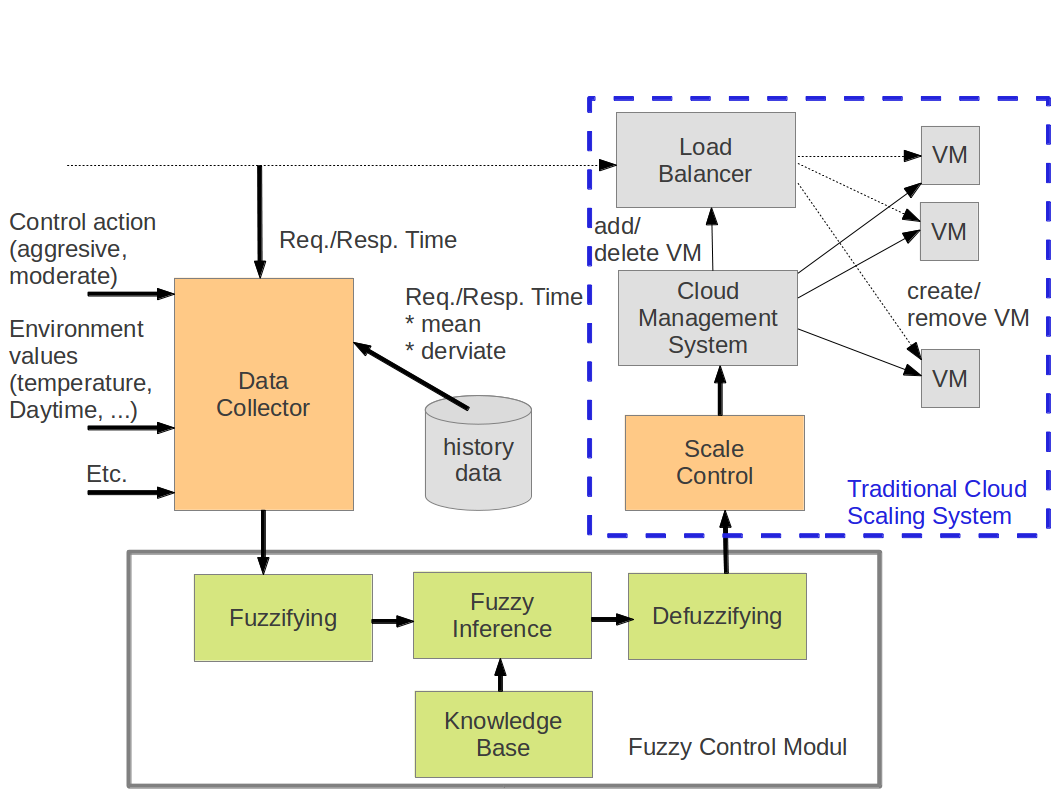
\includegraphics[width=0.7\textwidth]{chapters/chapter3/fig/architecture.png}
% \caption{QoS Fuzzy Control Architecture from  \cite{fuzzyQoS} }
% \label{fig:fuzzy}
% \end{center}
% \end{figure}
%
% The aim of the research was to show how a common cloud computing scaling service could be enabled to guarantee QoS parameters. Figure \ref{fig:fuzzy} shows the proposed architecture for enabling QoS control by Fuzzy rules. As proof of concept several test were performed in order to prove the effectiveness of each approach. Results showed that this method of controlling a cloud QoS parameter, in this particular case the request-response time, can result in significant less SLA violations. This marks a first step towards QoS control in the cloud, but additional parameters have to be tested on whether or not and by which methods they can be adjusted.

 
 
  \section{Conclusion}
In this chapter the current Cloud SLA landscape and developments towards SLA for cloud services have been presented. The general SLA management process and its adoption to the cloud computing model has been outlined. It could be shown that SLAs and QoS in the cloud have not yet been implemented sufficiently extensively. This is due to the lack of translation of performance metrics into SLAs and to the magical management of such KPIs. Cloud providers are unable to provide customers with extensive and detailed SLAs, as these require automated management of the resources and relevant set screws for the metrics. In addition, the transparent and intercompatible description of such cloud SLAs poses a problem, as there are various standards for describing and disagreeing with the content and scope of such cloud SLAs. Although recent efforts have been made to standardize this, there is no general standard yet.

